% How the global random state takes part when a function that draws three times is
% traced and called: the function; the graph jit() traces from it, with the
% part that implements the random state in blue; the program's view of the
% random state; its host object; and numbered notes on what happens.
% Build: see figures/README.md
\documentclass[tikz, border = 6pt]{standalone}
\usepackage[T1]{fontenc}
\usepackage{lmodern}
\usetikzlibrary{positioning, calc, fit, backgrounds, matrix}

\definecolor{keep}{HTML}{2A7AB0}

% The part of the graph that implements the side effect.
\newcommand{\se}[1]{\textcolor{keep}{#1}}
\newcommand{\cd}[1]{\texttt{#1}}

\tikzset{
  badge/.style = {circle, fill = black!65, text = white, font = \sffamily\tiny\bfseries,
    inner sep = 0pt, minimum size = 3.2mm, anchor = base},
  lines/.style = {matrix of nodes, row sep = {3.9mm, between origins}, column sep = 2pt,
    nodes = {anchor = base west, inner sep = 0.5pt, font = \ttfamily\scriptsize},
    column 2/.style = {nodes = {badge}}, column 3/.style = {nodes = {badge}}},
  fields/.style = {matrix of nodes, row sep = {3.9mm, between origins}, column sep = 2pt,
    nodes = {anchor = base west, inner sep = 0.5pt, font = \ttfamily\scriptsize},
    column 1/.style = {nodes = {text = black!55}}},
  box/.style = {rounded corners = 2pt, inner sep = 5pt},
  head/.style = {font = \footnotesize\bfseries, text = black!70, anchor = south west,
    inner sep = 1pt},
  note/.style = {font = \footnotesize, align = left, text width = 8.6cm, anchor = north west,
    inner sep = 0pt, execute at begin node = {\thickmuskip = 5mu}}
}

% A note: its text at #2, numbered #1 in a badge hanging to its left.
\newcommand{\note}[3]{
  \node[note] (#1) at #2 {#3};
  \node[badge, font = \sffamily\scriptsize\bfseries, minimum size = 3.8mm, anchor = north east]
    at ($(#1.north west) + (-0.15, 0.04)$) {#1};
}

\begin{document}
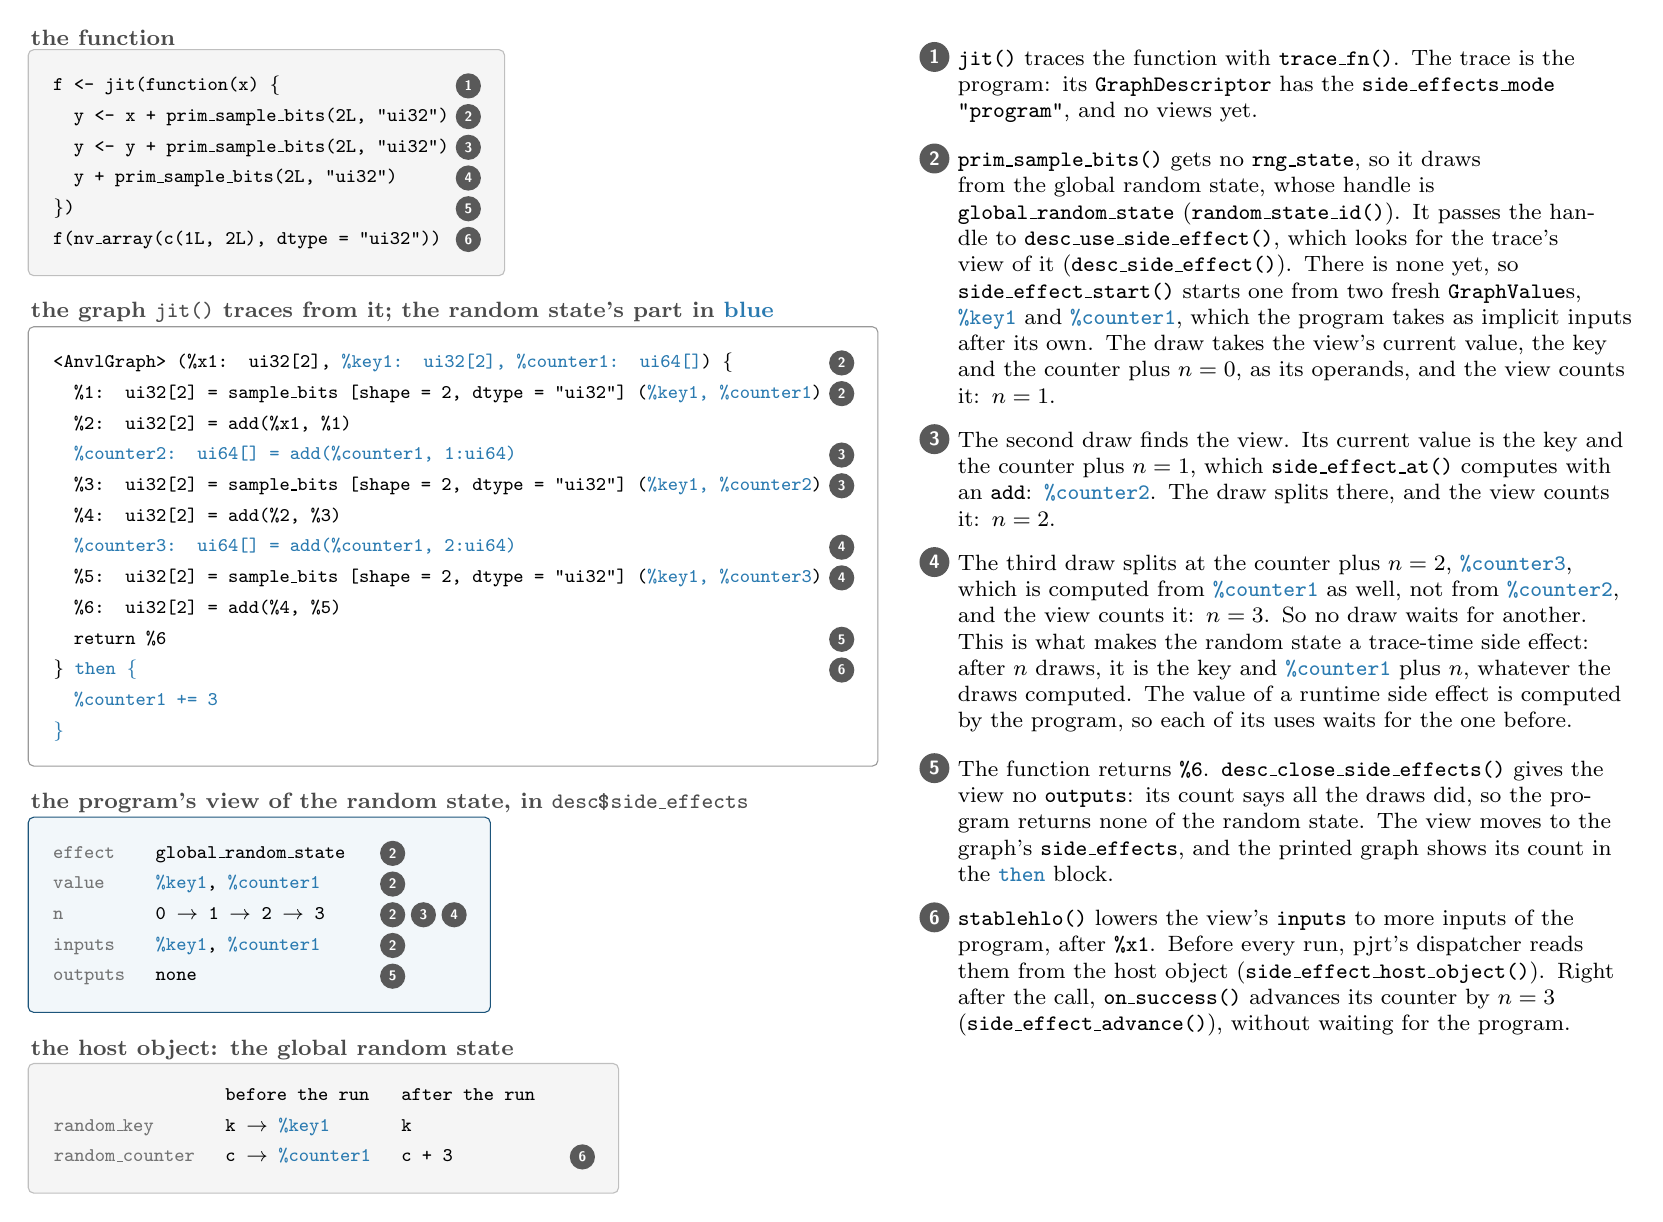
\begin{tikzpicture}

  \matrix[lines] (code) at (0, 0) {
    f <- jit(function(x) \{ & 1 \\
    \ \ y <- x + prim\_sample\_bits(2L, "ui32") & 2 \\
    \ \ y <- y + prim\_sample\_bits(2L, "ui32") & 3 \\
    \ \ y + prim\_sample\_bits(2L, "ui32") & 4 \\
    \}) & 5 \\
    f(nv\_array(c(1L, 2L), dtype = "ui32")) & 6 \\
  };
  \begin{scope}[on background layer]
    \node[box, draw = black!25, fill = black!4, fit = (code)] (codebox) {};
  \end{scope}
  \node[head] at (codebox.north west) {the function};

  \matrix[lines, below = 1.0 of code.south west, anchor = north west] (graph) {
    <AnvlGraph> (\%x1: ui32[2], \se{\%key1: ui32[2], \%counter1: ui64[]}) \{ & 2 \\
    \ \ \%1: ui32[2] = sample\_bits [shape = 2, dtype = "ui32"] (\se{\%key1, \%counter1}) & 2 \\
    \ \ \%2: ui32[2] = add(\%x1, \%1) & \\
    \ \ \se{\%counter2: ui64[] = add(\%counter1, 1:ui64)} & 3 \\
    \ \ \%3: ui32[2] = sample\_bits [shape = 2, dtype = "ui32"] (\se{\%key1, \%counter2}) & 3 \\
    \ \ \%4: ui32[2] = add(\%2, \%3) & \\
    \ \ \se{\%counter3: ui64[] = add(\%counter1, 2:ui64)} & 4 \\
    \ \ \%5: ui32[2] = sample\_bits [shape = 2, dtype = "ui32"] (\se{\%key1, \%counter3}) & 4 \\
    \ \ \%6: ui32[2] = add(\%4, \%5) & \\
    \ \ return \%6 & 5 \\
    \} \se{then \{} & 6 \\
    \ \ \se{\%counter1 += 3} & \\
    \se{\}} & \\
  };
  \begin{scope}[on background layer]
    \node[box, draw = black!40, fit = (graph)] (graphbox) {};
  \end{scope}
  \node[head] at (graphbox.north west)
    {the graph \cd{jit()} traces from it; the random state's part in \se{blue}};

  \matrix[fields, below = 1.0 of graph.south west, anchor = north west] (view) {
    effect &[8pt] global\_random\_state &[10pt] |[badge]| 2 \\
    value & \se{\%key1}, \se{\%counter1} & |[badge]| 2 \\
    n & 0 $\to$ 1 $\to$ 2 $\to$ 3 & |[badge]| 2 & |[badge]| 3 & |[badge]| 4 \\
    inputs & \se{\%key1}, \se{\%counter1} & |[badge]| 2 \\
    outputs & none & |[badge]| 5 \\
  };
  \begin{scope}[on background layer]
    \node[box, draw = keep!70!black, fill = keep!6, fit = (view)] (viewbox) {};
  \end{scope}
  \node[head] at (viewbox.north west)
    {the program's view of the random state, in \cd{desc\$side\_effects}};

  \matrix[fields, below = 1.0 of view.south west, anchor = north west] (host) {
    &[8pt] before the run &[8pt] after the run \\
    random\_key & k $\to$ \se{\%key1} & k \\
    random\_counter & c $\to$ \se{\%counter1} & c + 3 &[10pt] |[badge]| 6 \\
  };
  \begin{scope}[on background layer]
    \node[box, draw = black!25, fill = black!4, fit = (host)] (hostbox) {};
  \end{scope}
  \node[head] at (hostbox.north west) {the host object: the global random state};

  \coordinate (notes) at ($(codebox.north -| graphbox.east) + (1.0, 0)$);
  \note{1}{(notes)}
    {\cd{jit()} traces the function with \cd{trace\_fn()}. The trace is the program: its
     \cd{GraphDescriptor} has the \cd{side\_effects\_mode} \cd{"program"}, and no views yet.}
  \note{2}{($(1.south west) + (0, -0.35)$)}
    {\cd{prim\_sample\_bits()} gets no \cd{rng\_state}, so it draws from the global random
     state, whose handle is \cd{global\_random\_state} (\cd{random\_state\_id()}). It passes
     the handle to \cd{desc\_use\_side\_effect()}, which looks for the trace's view of it
     (\cd{desc\_side\_effect()}). There is none yet, so \cd{side\_effect\_start()} starts one
     from two fresh \cd{GraphValue}s, \se{\cd{\%key1}} and \se{\cd{\%counter1}}, which the
     program takes as implicit inputs after its own. The draw takes the view's current
     value, the key and the counter plus $n = 0$, as its operands, and the view counts it:
     $n = 1$.}
  \note{3}{($(2.south west) + (0, -0.35)$)}
    {The second draw finds the view. Its current value is the key and the counter plus
     $n = 1$, which \cd{side\_effect\_at()} computes with an \cd{add}: \se{\cd{\%counter2}}.
     The draw splits there, and the view counts it: $n = 2$.}
  \note{4}{($(3.south west) + (0, -0.35)$)}
    {The third draw splits at the counter plus $n = 2$, \se{\cd{\%counter3}}, which is
     computed from \se{\cd{\%counter1}} as well, not from \se{\cd{\%counter2}}, and the view
     counts it: $n = 3$. So no draw waits for another. This is what makes the random state a
     trace-time side effect: after $n$ draws, it is the key and \se{\cd{\%counter1}} plus
     $n$, whatever the draws computed. The value of a runtime side effect is computed by the
     program, so each of its uses waits for the one before.}
  \note{5}{($(4.south west) + (0, -0.35)$)}
    {The function returns \cd{\%6}. \cd{desc\_close\_side\_effects()} gives the view no
     \cd{outputs}: its count says all the draws did, so the program returns none of the
     random state. The view moves to the graph's \cd{side\_effects}, and the printed graph
     shows its count in the \se{\cd{then}} block.}
  \note{6}{($(5.south west) + (0, -0.35)$)}
    {\cd{stablehlo()} lowers the view's \cd{inputs} to more inputs of the program, after
     \cd{\%x1}. Before every run, pjrt's dispatcher reads them from the host object
     (\cd{side\_effect\_host\_object()}). Right after the call, \cd{on\_success()} advances
     its counter by $n = 3$ (\cd{side\_effect\_advance()}), without waiting for the
     program.}

\end{tikzpicture}
\end{document}
